\documentclass[12pt]{iopart}
\newcommand{\gguide}{{\it Preparing graphics for IOP Publishing journals}}
\usepackage{graphicx}
\graphicspath{{./figures/}}
\usepackage{setstack}
\bibliographystyle{iopart-num}
\usepackage{citesort}

\begin{document}

\title{Thermal reflow simulation of PMMA structures with non-uniform viscosity profile}
\author{F A Sidorov, A E Rogozhin}
\address{Valiev Institute of Physics and Technology, Russian Academy of Sciences, Moscow, 117218 Russia}
\ead{sidorov@ftian.ru}

\vspace{10pt}

\begin{abstract}
This paper presents a new approach to simulation of thermal viscoelastic reflow of e-beam exposed polymethyl methacrylate (PMMA) taking into account its non-uniform viscosity profile.
This approach is based on numerical ``soapfilm'' modeling of surface evolution, processed by free software ``Surface Evolver'' in area normalization mode.
PMMA viscosity profile is calculated by simulation of exposed PMMA number average molecular weight distribution using Monte-Carlo method and empirical equations.
The relation between PMMA viscosity and mobility of PMMA surface vertices was determined by thermal reflow simulation of uniform PMMA gratings using both analytical and numerical approaches in wide viscosity range.
The agreement between reflowed profiles simulated by these two approaches emphasizes the applicability of ``soapfilm'' modeling to simulation of polymer thermal reflow. 
The inverse mobility of PMMA surface vertices appeared to be proportional to PMMA viscosity with high accuracy.
The developed algorithm enables thermal reflow simulation of complex non-uniform structures, which allows the usage of predictable reflow as a stage of 3D microfabrication.
\end{abstract}

\vspace{2pc}

\noindent{\it Keywords}: grayscale e-beam lithography, non-uniform viscosity profile, thermal reflow

\actuality

Формирование трехмерных микро- и наноструктур является востребованным во множестве областей, таких как микроэлектроника, дифракционная оптика и нанофотоника, микро- и нанофлюидика и др. В настоящее время существует множество подходов к решению этой задачи, однако такие преимущества метода, как универсальность, высокая производительность и доступность зачастую оказываются взаимоисключающими. Универсальные методы с высоким разрешением (например, полутоновая литография~\cite{GL_general}, двухфотонная литография~\cite{TPL_castle} или сканирующая зондовая литография~\cite{SPL_mechanical}) требуют использования сложного высокоточного оборудования и обладают при этом достаточно низкой производительностью. Более производительные и доступные методы позволяют получить только периодические структуры (интерференционная литография~\cite{IL_metamaterials}), либо структуры определенного вида (наноимпринтная литография~\cite{NIL_1}). Таким образом, в настоящее время отсутствует метод получения произвольных микро- и наноструктур, являющийся одновременно высокопроизводительным и простым в реализации.

Ввиду этого внимания заслуживает метод сухого электронно-лучевого травления резиста (СЭЛТР) –- относительно новый одностадийный литографический метод формирования рельефа в слое позитивного резиста, основанный на цепной реакции деполимеризации полимерного резиста и самопроявлении изображения непосредственно в процессе электронно-лучевого экспонирования резиста, проводимого при температурах выше его температуры стеклования~\cite{Bruk_2013, Bruk_2016_mee}. Отличительными особенностями метода являются исключительно высокая чувствительность резиста, высокое разрешение по вертикали и возможность формирование рельефа без этапа проявления, а также скругленные стенки профиля линии. Высокая чувствительность резиста обеспечивает производительность метода в сотни раз превышающую производительность обычной электронно-лучевой литографии. Благодаря этим особенностям метод может быть использован для формирования дифракционных оптических элементов, различных трехмерных микро- и наноструктур или масок. Также возможной областью его применения является формирование каналов для использования в микро- и нанофлюидике, поскольку отсутствие острых углов в сечении канала положительно скажется на его гидравлическом диаметре.

Однако, латеральное разрешение метода ограничено, и в настоящее время при использовании электронно-лучевых систем с диаметром электронного луча около 10-15 нм удается получать линии шириной около 300 нм. Область применения метода могла бы быть существенно расширена, если бы удалось повысить его латеральное разрешение. В силу одновременного протекания в процессе СЭЛТР множества различных процессов точный механизм формирования конечного профиля линии не был понятен, что не позволяло выявить пути оптимизации данного метода. Таким образом, целесообразным является разработка физической модели метода СЭЛТР, что позволит определить возможности метода и оптимизировать его для применения в различных областях.


\previouswork

Первые шаги в изучении метода микролитографии на основе термической деполимеризации резиста описываются в работе~\cite{Bruk_2000}. В ней приводятся результаты инициированной $\gamma$-излучением деполимеризации ПММА в виде нанометрового слоя, адсорбированного на поверхности пор силохрома. Несмотря на то, что в данной работе термическая деполимеризация не использовалась для формирования структуры в резисте, а исследовалась в общем, результаты работы позволили определить особенности потенциально возможного метода микроструктурирования на основе этого явления. Так, например, были получены оценки для времени диффузии мономера в слое ПММА после разрушения молекулы и длины кинетической цепи деполимеризации, сделаны выводы о масштабах протекания процессов передачи активного центра деполимеризации на мономер и полимер. Также было установлено, что при термической деполимеризации ПММА при температурах 120--180 $^\circ$C влияние процессов реполимеризации пренебрежимо мало.

Впоследствии были проведены эксперименты по изучению термической деполимеризации полиметилметакрилата (ПММА), протекающей при экспонировании электронным лучом, а также впервые были продемонстрированы двумерные и трехмерные структуры, полученные в ПММА в этом процессе~\cite{Bruk_2013}.

Наиболее актуальные на сегодняшний день экспериментальные результаты по исследованию метода сухого электронно-лучевого травления резиста приведены в работах~\cite{Bruk_2015_co, Bruk_2016_mee}. Помимо вышеописанных ступенчатых профилей, в этих работах исследовались периодические профили, полученные при экспонировании резиста электронным лучом вдоль серии параллельных линий (рисунок~\ref{fig:DEBER_many_profiles}). Было продемонстрировано, что при таком экспонировании результирующий профиль приобретает практически синусоидальную форму, что является аргументом в пользу применения метода СЭЛТР для формирования некоторых дифракционных оптических элементов~\cite{Mitreska_sin_gratings}. При этом снова была отмечена высокая производительность метода -- при температуре 160 $^\circ$C полное травление в центре линии было достигнуто при дозе экспонирования менее 1 мкКл/см$^2$. Также была продемонстрирована возможность достаточно точного переноса профиля, полученного в ПММА, на поверхность вольфрама и кремния за счет сухого травления в реакторе индуктивно-связанной плазмы (рисунок~\ref{fig:DEBER_Si_W}). Этот факт теоретически позволяет использовать метод СЭЛТР для формирования, например, штампов для термической наноимпринтной литографии.


\aimsandtasks\ 

Целью данной работы является определение и исследование основных процессов, протекающих при сухом электронно-лучевом травлении резиста, а также создание физической модели метода СЭЛТР, позволяющей определить результирующий профиль линии при различных условиях экспонирования. В большинстве экспериментов, которые были проведены для исследования метода СЭЛТР, в качестве резиста и материала подложки использовались ПММА и Si, соответственно. Учитывая также тот факт, что свойства ПММА достаточно хорошо изучены, при создании модели процесса СЭЛТР в рамках данной работы в качестве резиста рассматривался именно этот материал. Для достижения поставленной цели необходимо было решить следующие задачи:

\begin{enumerate}
  \item На основе существующих моделей взаимодействия электронного излучения с веществом реализовать детальный алгоритм моделирования рассеяния электронного пучка в системе ПММА/Si;
  \item Определить механизмы, приводящие к разрыву молекул ПММА при экспонировании в условиях повышенной температуры;
  \item Разработать алгоритм моделирования электронно-стимулированной деструкции молекул ПММА при температурах метода СЭЛТР;
  \item Разработать модель процесса изменения распределения молекулярной массы ПММА при экспонировании;
  \item Определить температурную зависимость длины кинетической цепи при деполимеризации ПММА в условиях метода СЭЛТР;
  \item Разработать модель диффузии в слое ПММА мономеров, образовавшихся в процессе деполимеризации;
  \item Реализовать алгоритм моделирования растекания линии, вызванного пониженной вязкостью ПММА при температурах процесса СЭЛТР;
  \item Разработать программу моделирования метода СЭЛТР с учетом совместное протекание процессов рассеяния электронного пучка, деполимеризации, диффузии мономеров и растекания профиля линии;
  \item На основе разработанного алгоритма моделирования определить пути оптимизации разрешения метода СЭЛТР.
\end{enumerate}


\defpositions

\begin{enumerate}
	\item При комнатной температуре электронно-стимулированная деструкция ПММА протекает за счет взаимодействия налетающего электрона с валентными электронами ММА, образующими связи между атомами углерода в главной цепи ПММА. Увеличение радиационно-химического выхода разрывов с ростом температуры может быть описано за счет увеличения вероятности разрыва главной цепи ПММА при разрыве связей между атомами водорода и атомами углерода, образующими главную цепи. При температурах в диапазоне от 30 °С до 160 °С данная вероятность увеличивается практически линейно от 0 до 1.
	\item Область оптимальных температур для метода СЭЛТР составляет 120-160 °С. Кинетическая длина цепи при деполимеризации ПММА в этой области изменяется от 500 до 3200 с ростом температуры, при этом имеет место передача активного центра деполимеризации с мономера на полимер;
	\item При использовании в методе СЭЛТР слоев ПММА толщиной до 1 мкм процессы диффузии мономера в слое ПММА не замедляют процесс формирования рельефа;
	\item При экспонировании вдоль серии линий при длительном суммарном времени нагрева форма профиля линии приближается к синусоидальной. Увеличение разрешения метода СЭЛТР может быть достигнуто за счет уменьшения суммарного времени нагрева, до значений, сопоставимых с временем затухания гармоник в фурье-образе профиля линии с высокими частотами (n > 10).
\end{enumerate}


\novelty

\begin{enumerate}
  \item Впервые предложена количественная модель, описывающая электронно-стимулированную деструкция молекул ПММА на молекулярном уровне с учетом температурного эффекта;
  \item Впервые исследовано совместное протекание процессов рассеяния электронного пучка в полимерном резисте, деполимеризация резиста, диффузия продуктов распада молекул резиста и растекание профиля;
  \item Впервые проведено моделирование профиля линии, получаемой методом сухого электронно-лучевого травления резиста.
\end{enumerate}


\influence\

Теоретическая значимость работы состоит в том, что впервые была создана модель формирования рельефа в резисте за счет совместного воздействия основных процессов, характерных для метода СЭЛТР – электронно-стимулированной деструкции резиста при повышенных температурах, термической деполимеризации резиста, диффузии мономеров слое резиста и растекания профиля линии за счет пониженной вязкости. Практическая значимость работы заключается в том, что был разработан алгоритм, позволяющий промоделировать форму профиля линии, получаемой методом СЭЛТР при различных условиях экспонирования и определить оптимальные условия для каждой конкретной задачи.


\methods\

Основным методом исследования основных процессов СЭЛТР являлось математическое моделирование; Для моделирования рассеяния электронного пучка использовался Монте-Карло алгоритм с дискретными потерями энергии. Моделирование слоя ПММА производилось на основе модели идеальной цепи; Моделирование диффузии мономера в слое ПММА проводилось на основе Монте-Карло алгоритма, длины свободного пробега мономеров определялись из функции Грина задачи диффузии частицы в свободном пространстве; Для моделирования растекания профиля линии применялось фурье-преобразование профиля с дальнейшим определением времени затухания различных гармоник из двумерного уравнения Навье-Стокса и уравнения непрерывности в условиях отсутствия скольжения с учетом давления Лапласа и расклинивающего давления.


\probation\

Поскольку на конечный профиль линии, получаемой методом СЭЛТР, влияет сразу несколько процессов, точность их описания проверялась на каждом этапе. Так, при моделировании рассеяния электронного пучка в системе ПММА/Si сечения упругих и неупругих процессов вычислялись с использованием наиболее современных моделей взаимодействия излучения с веществом (моттовские дифференциальные сечения упругого рассеяния и сечения, полученные с использованием диэлектрической функции Мермина и модели обобщенных осцилляторов для неупругого рассеяния). Механизмы разрыва молекул ПММА при комнатной и повышенной температуре определялись на основе моделирования радиационно-химического выхода разрывов, вычисляемого экспериментально из распределения молекулярной массы. Полученные значения для длины кинетической цепи при деполимеризации ПММА при различных температурах согласуются с опубликованными значениями, рассчитанными на основе констант деполимеризации и обрыва кинетической цепи деполимеризации в кинетических моделях термической деструкции ПММА. Диффузия мономеров в слое ПММА моделировалась с коэффициентами диффузии, соответствующим различным температурам и массовой доле мономера в слое ПММА. Полученная в результате оценка сверху для времени диффузии привела к значению, пренебрежимо малому по сравнению с характерным временем протекания других процессов. Подход, использующийся для моделирования растекания профиля линии в процессе СЭЛТР, эффективно применяется в смежной области – моделировании растекания структур, полученных методом наноимпринтной литографии, и его точность отмечена в ряде работ. Все вышеперечисленное вкупе с соответствием между экспериментальными и промоделированными профилями обеспечивает достоверность полученных результатов.

Основные результаты работы докладывались на следующих конференциях:
\begin{itemize}
	\item 60-я всероссийская научная конференция МФТИ, Долгопрудный (2016);
	\item International conference on information technology and nanotechnology (ITNT), Самара (2017, 2018, 2020, 2022);
	\item III International Conference on modern problems in physics of surfaces and nanostructures (ICMPSN17), Ярославль (2017);
	\item Micro- and Nanoengineering (MNE), Копенгаген (2018), Родос (2019);
	\item International School and Conference "Saint-Petersburg OPEN"on Optoelectronics, Photonics, Engineering and Nanostructures, Санкт-Петербург (2019, 2020).	
\end{itemize}

Диссертация состоит из трёх глав, основные результаты которых изложены в статьях~\cite{my_CO, my_microlenses, my_evidence, my_detailed, my_review, my_MEE, my_Gvalue, my_microscopic, my_Isaev}. Все статьи опубликованы в рецензируемых международных журналах, включённых в библиографические базы (РИНЦ, Scopus, Web of Science).


\contribution\

Общая постановка задачи осуществлялась научным руководителем автора Рогожиным А. Е. Для верификации результатов моделирования были использованы структуры, полученные методом СЭЛТР М. А. Бруком, А. Е. Рогожиным и Е. Н. Жихаревым. Все результаты, изложенные настоящей диссертации, получены автором лично.

\section{Simulation of e-beam exposed PMMA viscosity profile}
In this study, thermal reflow is simulated for PMMA with non-uniform viscosity profile caused by e-beam exposure at room temperature.
According to equations~\ref{eq:WLF} and \ref{eq:3p4_3p1}, one can calculate PMMA viscosity for any specific temperature and number average molecular weight, so PMMA number average molecular weight distribution is of interest.
The distribution of PMMA local $M_n$ could be obtained by simulation of e-beam induced PMMA main-chain scissions.
For the latter, Monte-Carlo simulation of e-beam scattering in PMMA/Si structure was implemented.
Elastic scattering cross-section were obtained by relativistic partial wave expansion method (Mott cross-sections) using free software ``ELSEPA''~\cite{ELSEPA}.
Inelastic scattering was simulated using models based on energy loss functions of PMMA and Si, provided by Dapor~\cite{Dapor} and Valentin~\cite{Valentin}.
Next, according to Aktary~\cite{Aktary}, PMMA main-chain scissions were supposed occur due to inelastic electron-electron scattering.
Electron-electron scattering events, leading to PMMA main-chain scissions were simulated by Monte-Carlo technique with introducing the scission probability ($p_s$):
\begin{equation}
	\mathrm{electron-electron \ inelastic \ scattering: \ } \cases{\xi < p_s: & scission \\
		\xi \geq p_s: & no scission}
\end{equation}
where $\xi$ -- a random variable uniformly distributed on [0, 1).
Value of $p_s$ for room temperature (25 $^\circ$C) was determined by simulation of experimental radiation scission yield using the approach described in our previous paper~\cite{my_MEE} and compised 0.05.

Simulated PMMA main-chain scission events were stored in 3D histograms with 50~nm bin size.
The example of PMMA main-chain scission distribution simulated for line exposure using this approach is shown in Fig.~\ref{fig:sci_hist}.

\begin{figure}[h]
	\centering
	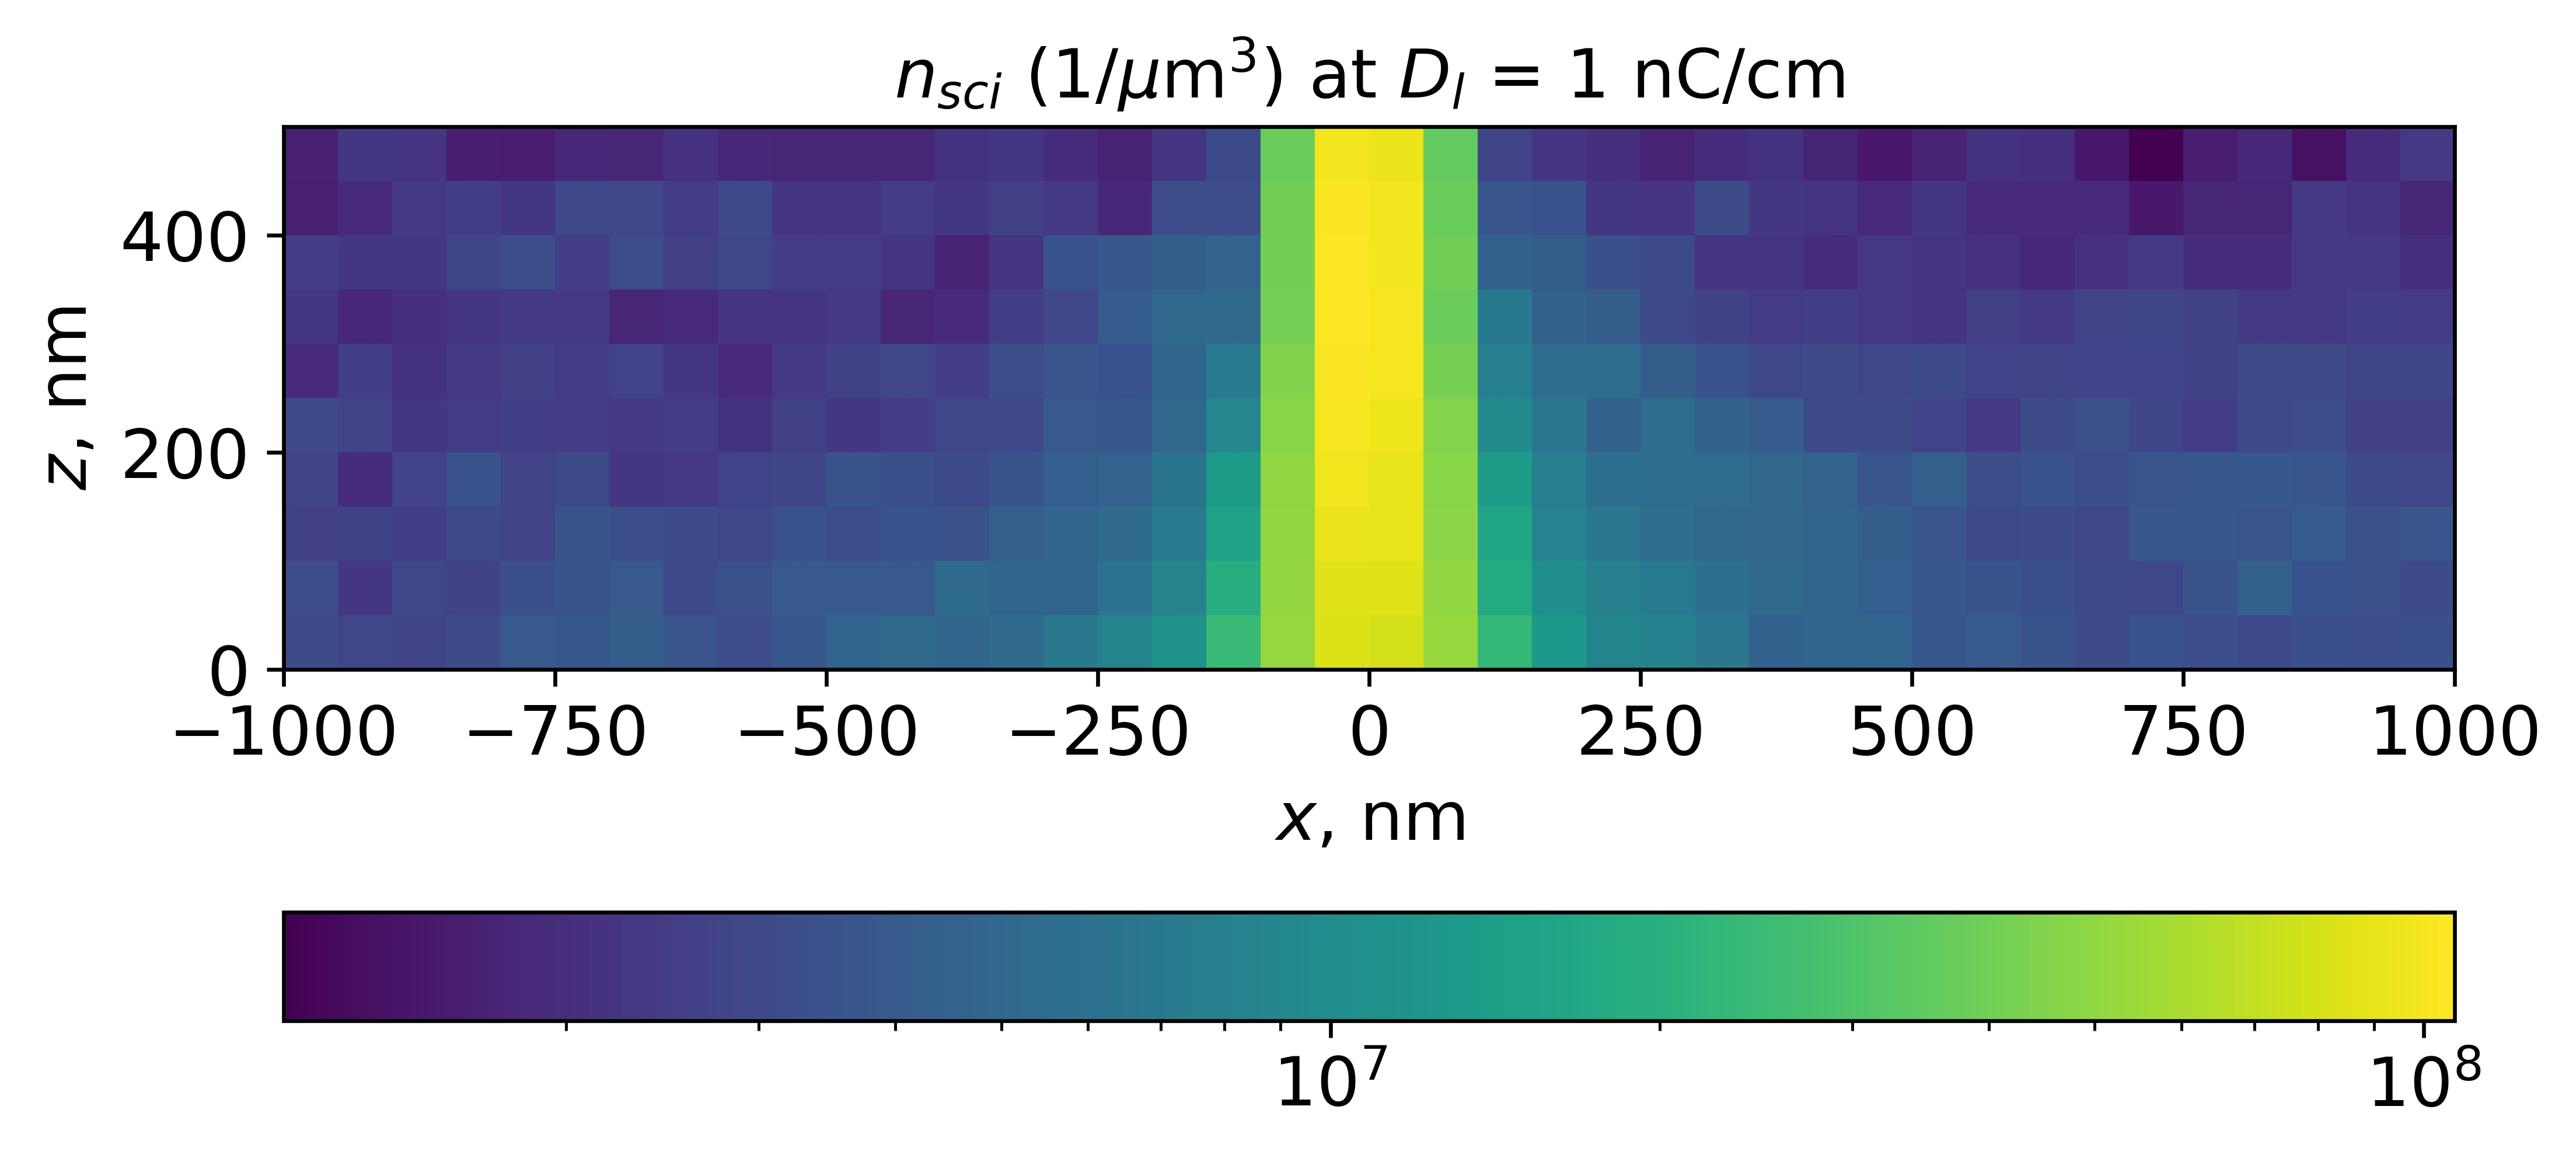
\includegraphics[width=0.8\linewidth]{sci_conc_1uC_cm_LOG}
	\caption{
		Simulation of local PMMA main-chain scission concentration in PMMA layer for line exposure.
		Line dose is 1 nC/cm, line width -- 300~nm, e-beam energy -- 20 keV, PMMA layer thickness -- 500 nm.
		Scission probability in inelastic electron-electron scattering is 0.05, which corresponds to room temperature (25$^\circ$C).
	}
	\label{fig:sci_hist}
\end{figure}

Then, number average molecular weight was calculated for each bin using the model of scissions randomly occurring at the bonds between the monomers~\cite{Ku1969}:
\begin{equation}
	\frac{1}{M_n^\prime} = \frac{w_s}{M_0} + \frac{1}{M_n},
\end{equation}
where $M_n$ and $M_n^\prime$ -- PMMA number average molecular weight before and after exposure, respectively, $M_0$ -- monomer molecular weight (100 for methyl methacrylate, MMA), $w_s$ -- probability of scission at a bond.
$w_s$ values were calculated for each bin using the formula:
\begin{equation}
	w_s = \frac{N_{sci}}{N_{mon}},
\end{equation}
where $N_{sci}$ -- number of scissions and $N_{mon}$ -- number of monomers in the bin, respectively.
Number of monomers in the bin of (50~nm)$^3$ size was calculated from PMMA density (1.19 g/cm$^3$) and MMA molecular weight (100 g/mol) and comprised 894809.
The example of $M_n^\prime$ distribution, simulated for line exposure by this method, is shown in Fig.~\ref{fig:Mn_hist}.

\begin{figure}
	\centering
	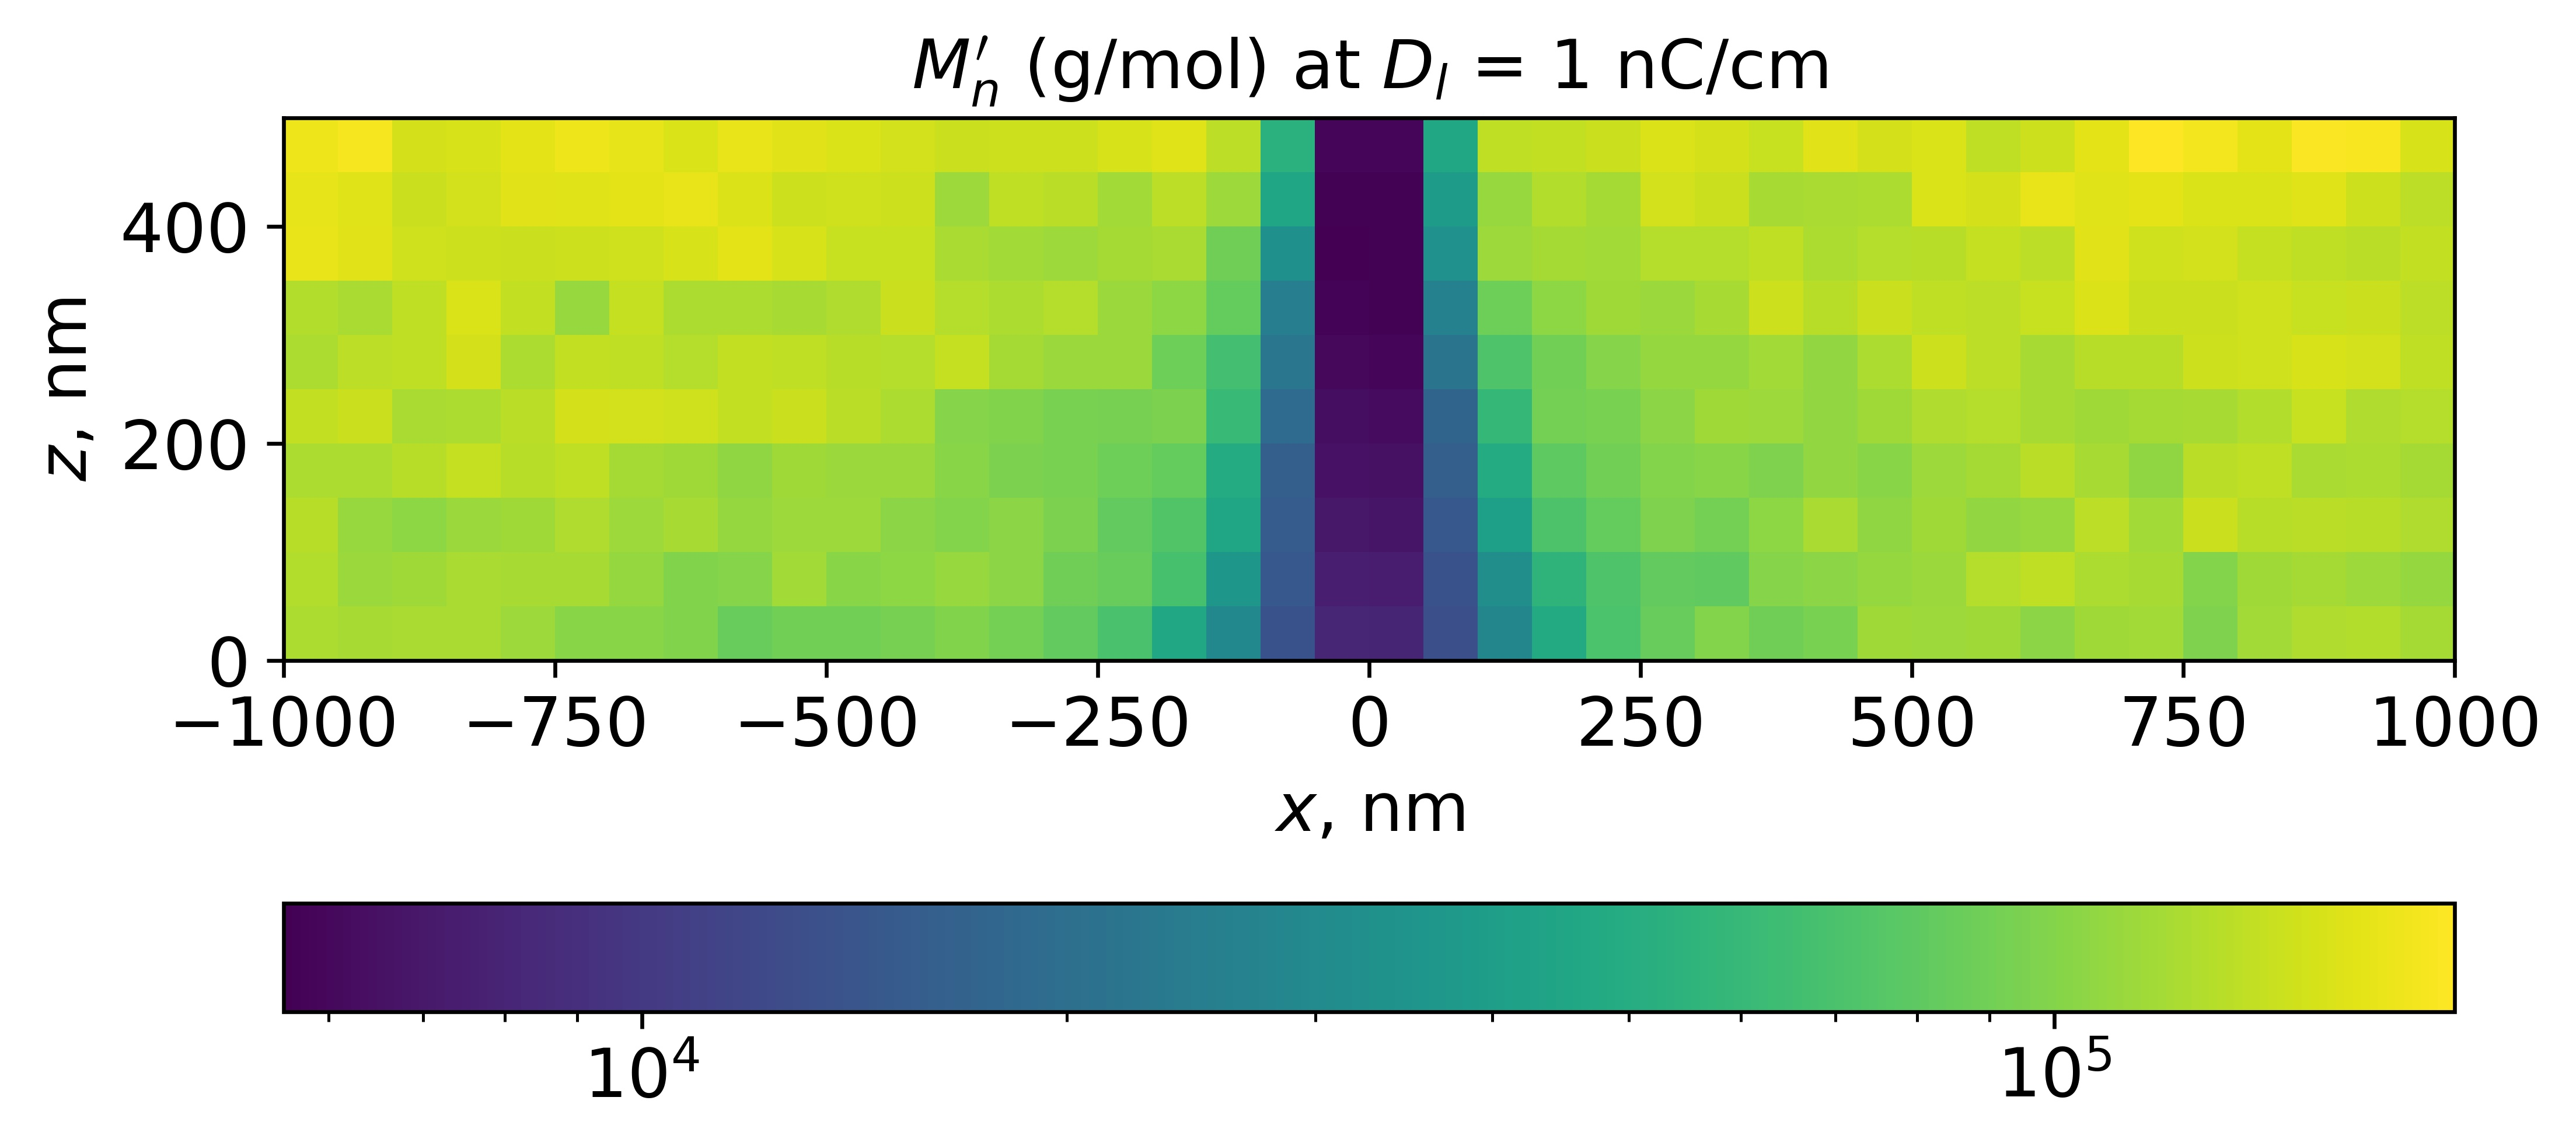
\includegraphics[width=0.8\linewidth]{Mn_prime_mat_easy_1_nC_cm_LOG}
	\caption{
		Simulation of local number average PMMA molecular weight in PMMA layer for line exposure at room temperature.
		Line dose is 1 nC/cm, line width -- 300~nm, e-beam energy -- 20 keV, PMMA layer thickness -- 500 nm.
		Initial PMMA number average molecular weight is 271000.
	}
	\label{fig:Mn_hist}
\end{figure}

Finally, local viscosity of exposed PMMA was calculated for required temperature using equation~\ref{eq:WLF} and for the following simulation viscosity distribution is averaged along $z$ axis (Fig.~\ref{fig:eta_arr}).

\begin{figure}
	\centering
	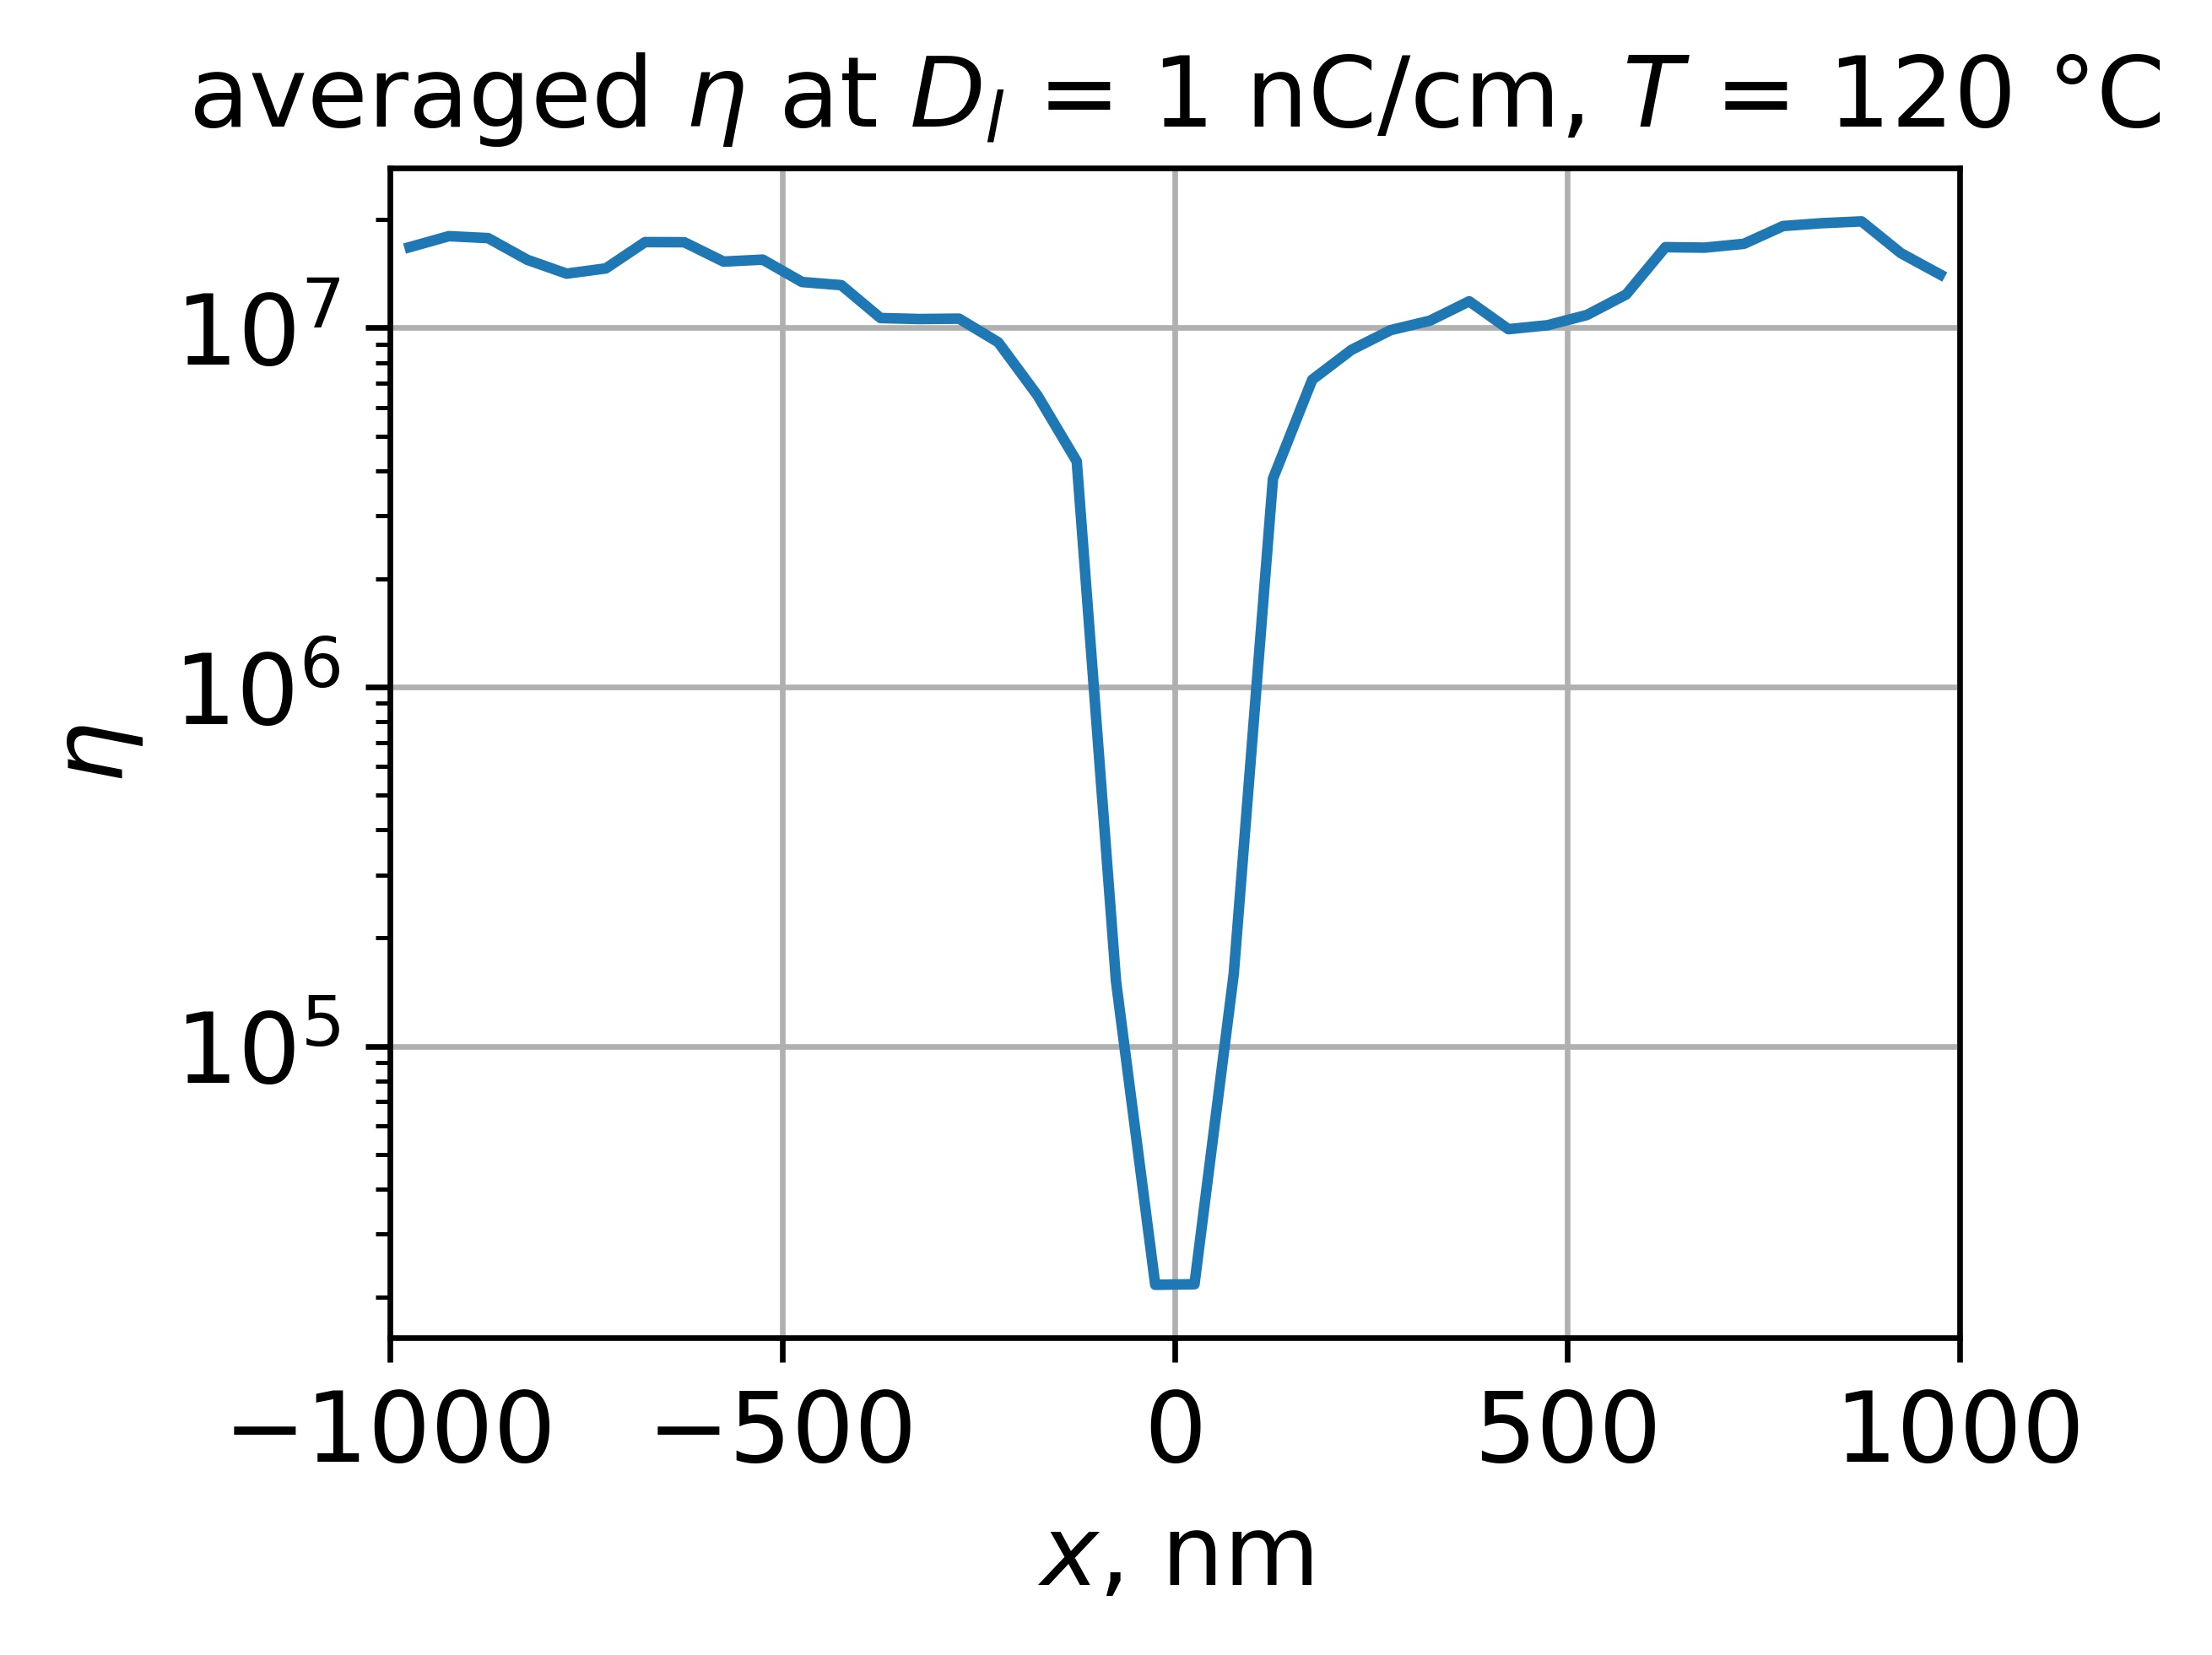
\includegraphics[width=0.6\linewidth]{eta_arr_1_nC_cm_120C_LOG}
	\caption{
			Simulation of averaged (along $z$ axis) viscosity profile in e-beam exposed PMMA layer for 120 $^\circ$C.
			Line dose is 1 nC/cm, e-beam energy -- 20 keV, PMMA layer thickness -- 500 nm.
			Initial PMMA number average molecular weight is 271000, PMMA reflow temperature is 120~$^\circ$C.
		}
	\label{fig:eta_arr}
\end{figure}

\section{Determination of e-beam exposed PMMA vertex mobilities}

Obtained PMMA viscosity profile couldn't be used for thermal reflow simulation so far -- the analytical approach based on profile Fourier transform could be applied in case of uniform viscosity only.
On the other hand, the numerical approach allows reflow simulation of non-uniform structures, but it bases on vertex mobilities, not viscosity.
Therefore, one should investigate the correlation between polymer viscosity and vertex mobilities of its surface.
For this purpose, thermal reflow was simulated by both approaches for the PMMA rectangular gratings, which parameters corresponded to Leveder study~\cite{Leveder_2010} -- 2 $\mu$m pitch and 28 nm depth.
First, for PMMA viscosity values in range 10$^2$--10$^6$ Pa$\cdot$s grating reflow was simulated analytically with constant time steps.
Then the grating surface was reconstructed in SE and surface evolution during grating reflow was simulated numerically with vertex mobility equal to 1.
During the numerical simulation, \textit{scale} values giving the same grating profiles as ones obtained using analytical approach, were determined (Fig.~\ref{fig:gratings_reflow}).
It was found that in the beginning of reflow there is a slight discrepancy between profiles simulated analytically and numerically but then both approaches lead to almost sinusoidal shape as it is predicted by equations~\ref{eq:Fourier_1},~\ref{eq:Fourier_2}~and~\ref{eq:Fourier_3}.
Time-\textit{scale} data obtained for different viscosity values showed almost direct proportionality between \textit{scale} and time ($t$) (Fig.~\ref{fig:alphas}):
\begin{equation} \label{eq:scale_alpha_t}
	scale \approx \alpha \cdot t.
\end{equation}
The values of $\alpha$ obtained by approximation of $t$-\textit{scale} data by a function~\ref{eq:scale_alpha_t} demonstrated quite linear dependence of $\ln(\alpha)$ on $\ln(\eta)$ (Fig.~\ref{fig:final_fit}).
The approximation of $\ln(\eta)$-$\ln(\alpha)$ data by the function
\begin{equation}
	\alpha = \frac{C}{\eta^\beta}
\end{equation}
resulted in $C$ and $\beta$ values equal to 26.142 and 0.989.
Thus, there is almost inverse proportionality between $\alpha$ and polymer viscosity:
\begin{equation}
	\alpha \approx \frac{26.142}{\eta}.
\end{equation}

\begin{figure}[h]
	\centering
	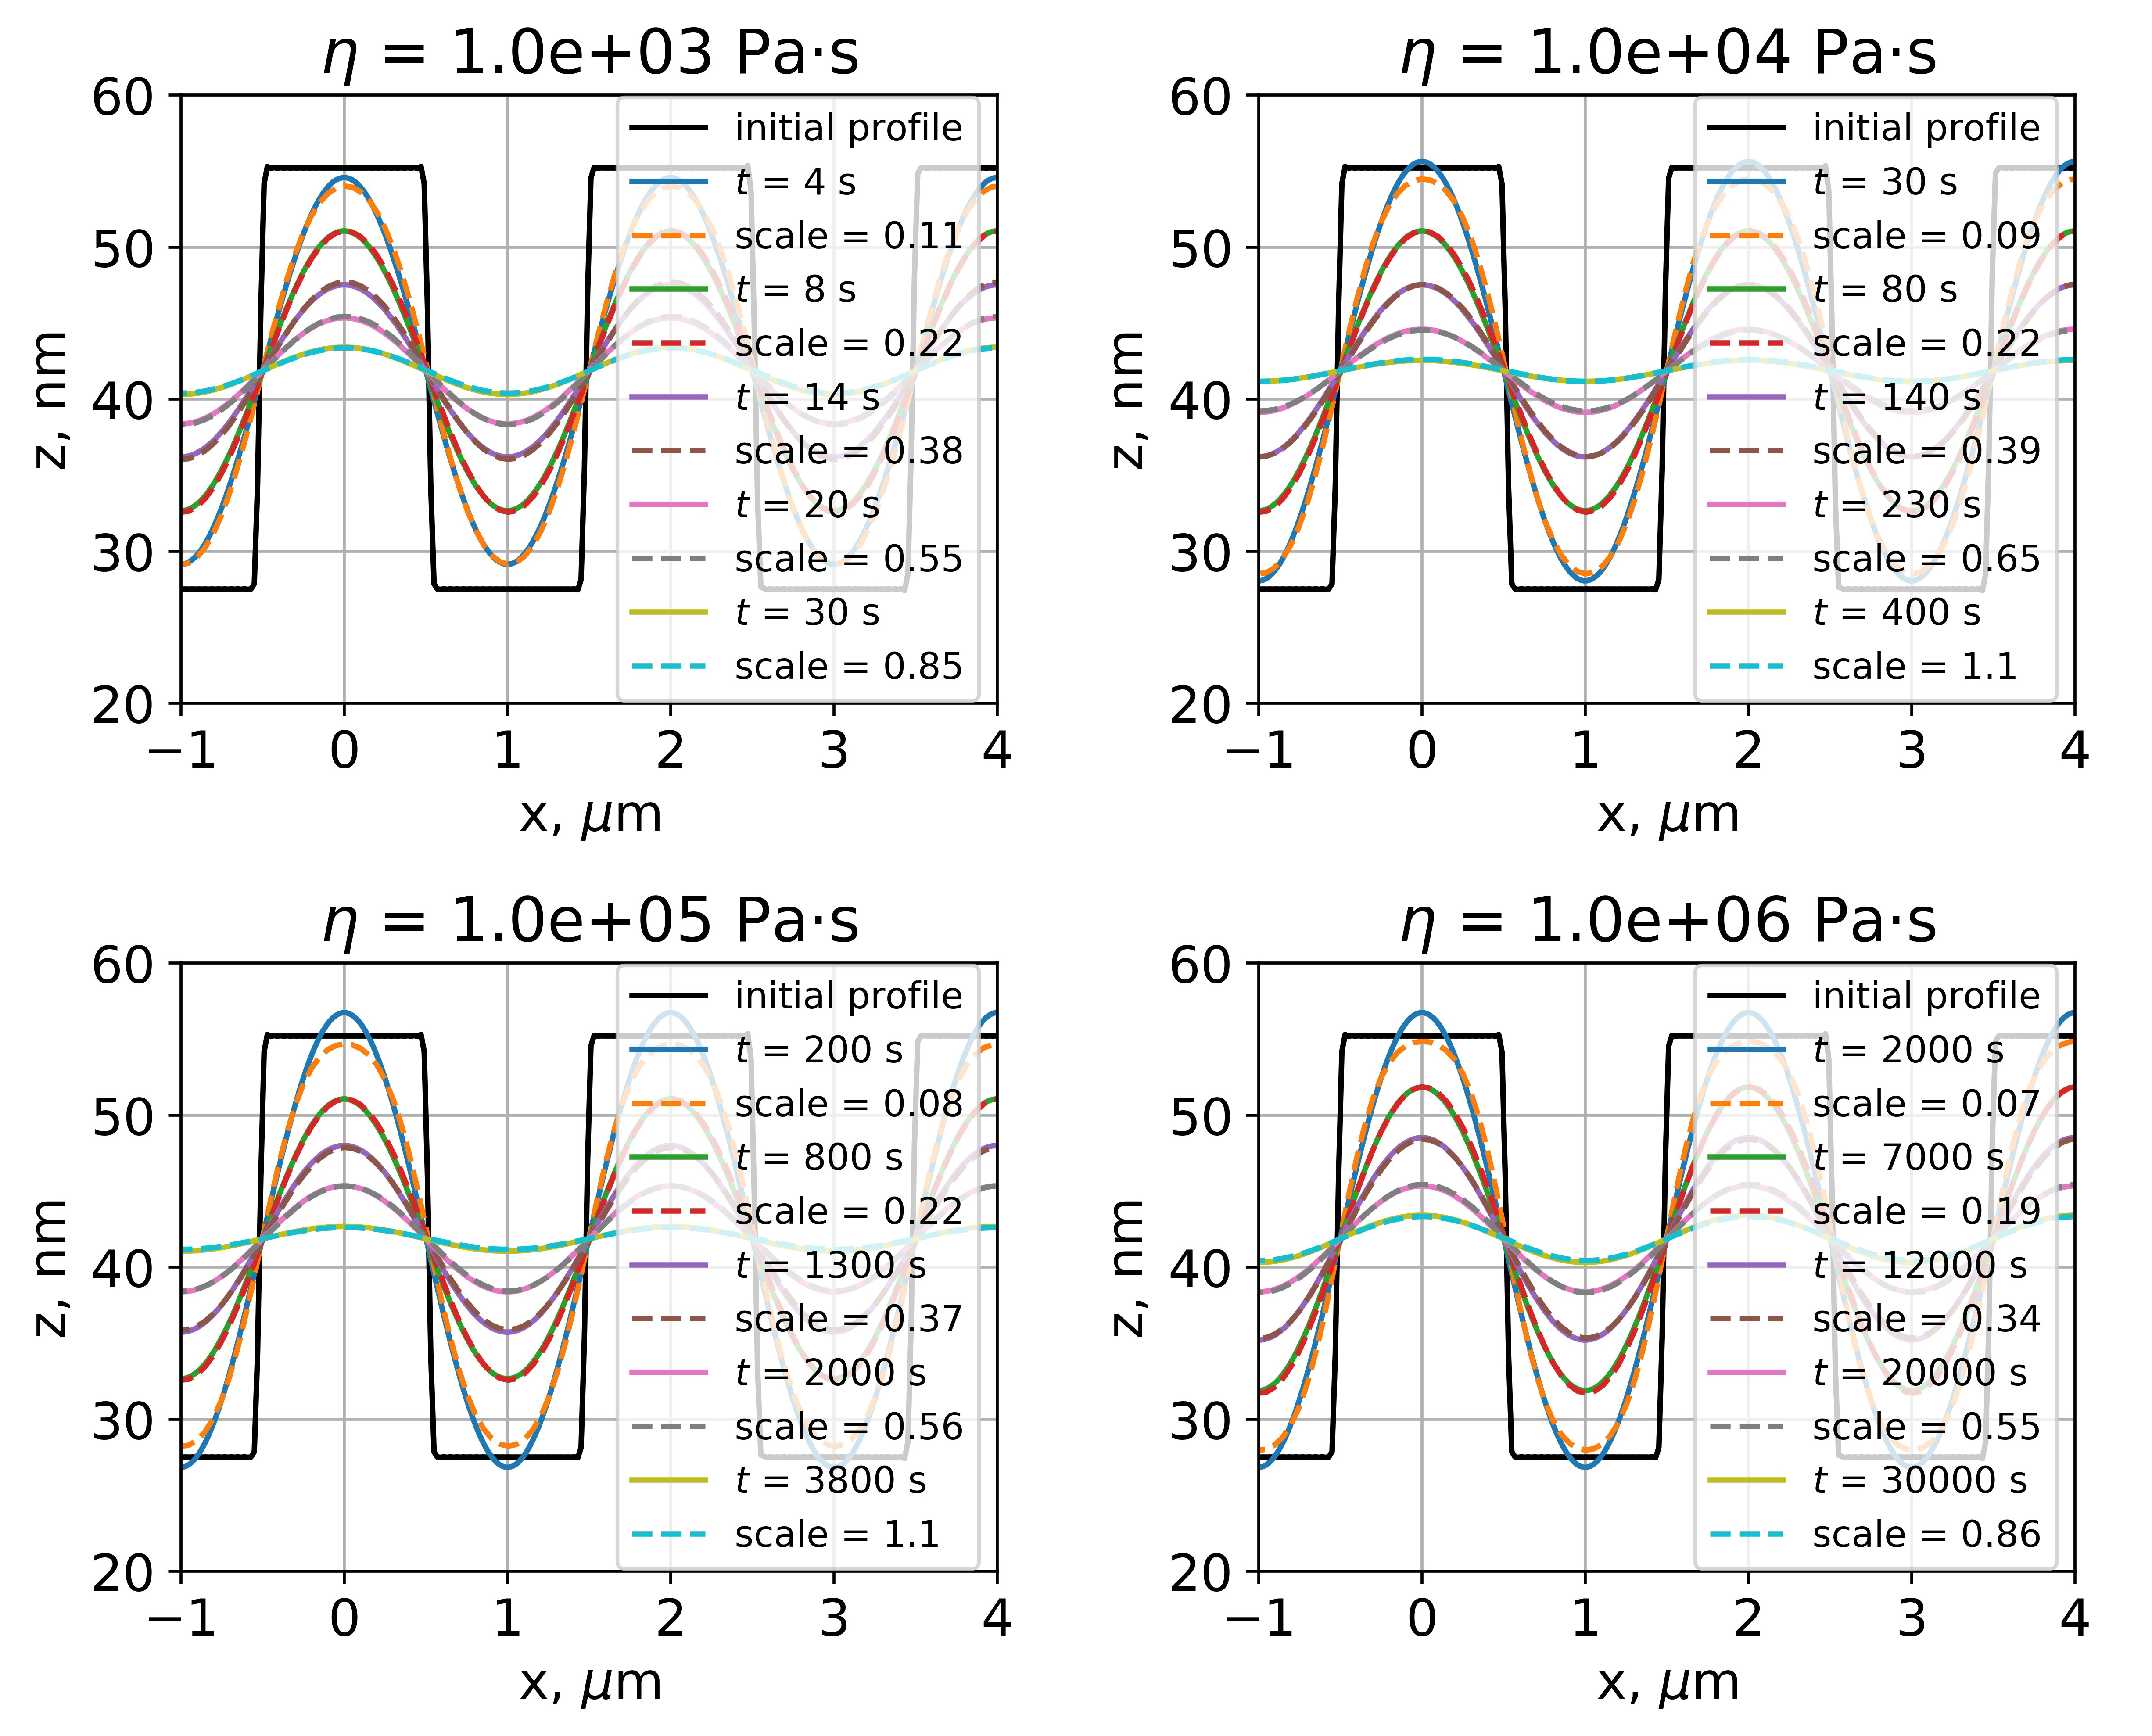
\includegraphics[width=\linewidth]{gratings_reflow}
	\caption{Thermal reflow of PMMA rectangular grating simulated by analytical and numerical approaches for different PMMA viscosity values.}
	\label{fig:gratings_reflow}
\end{figure}

\begin{figure}[h]
	\centering
	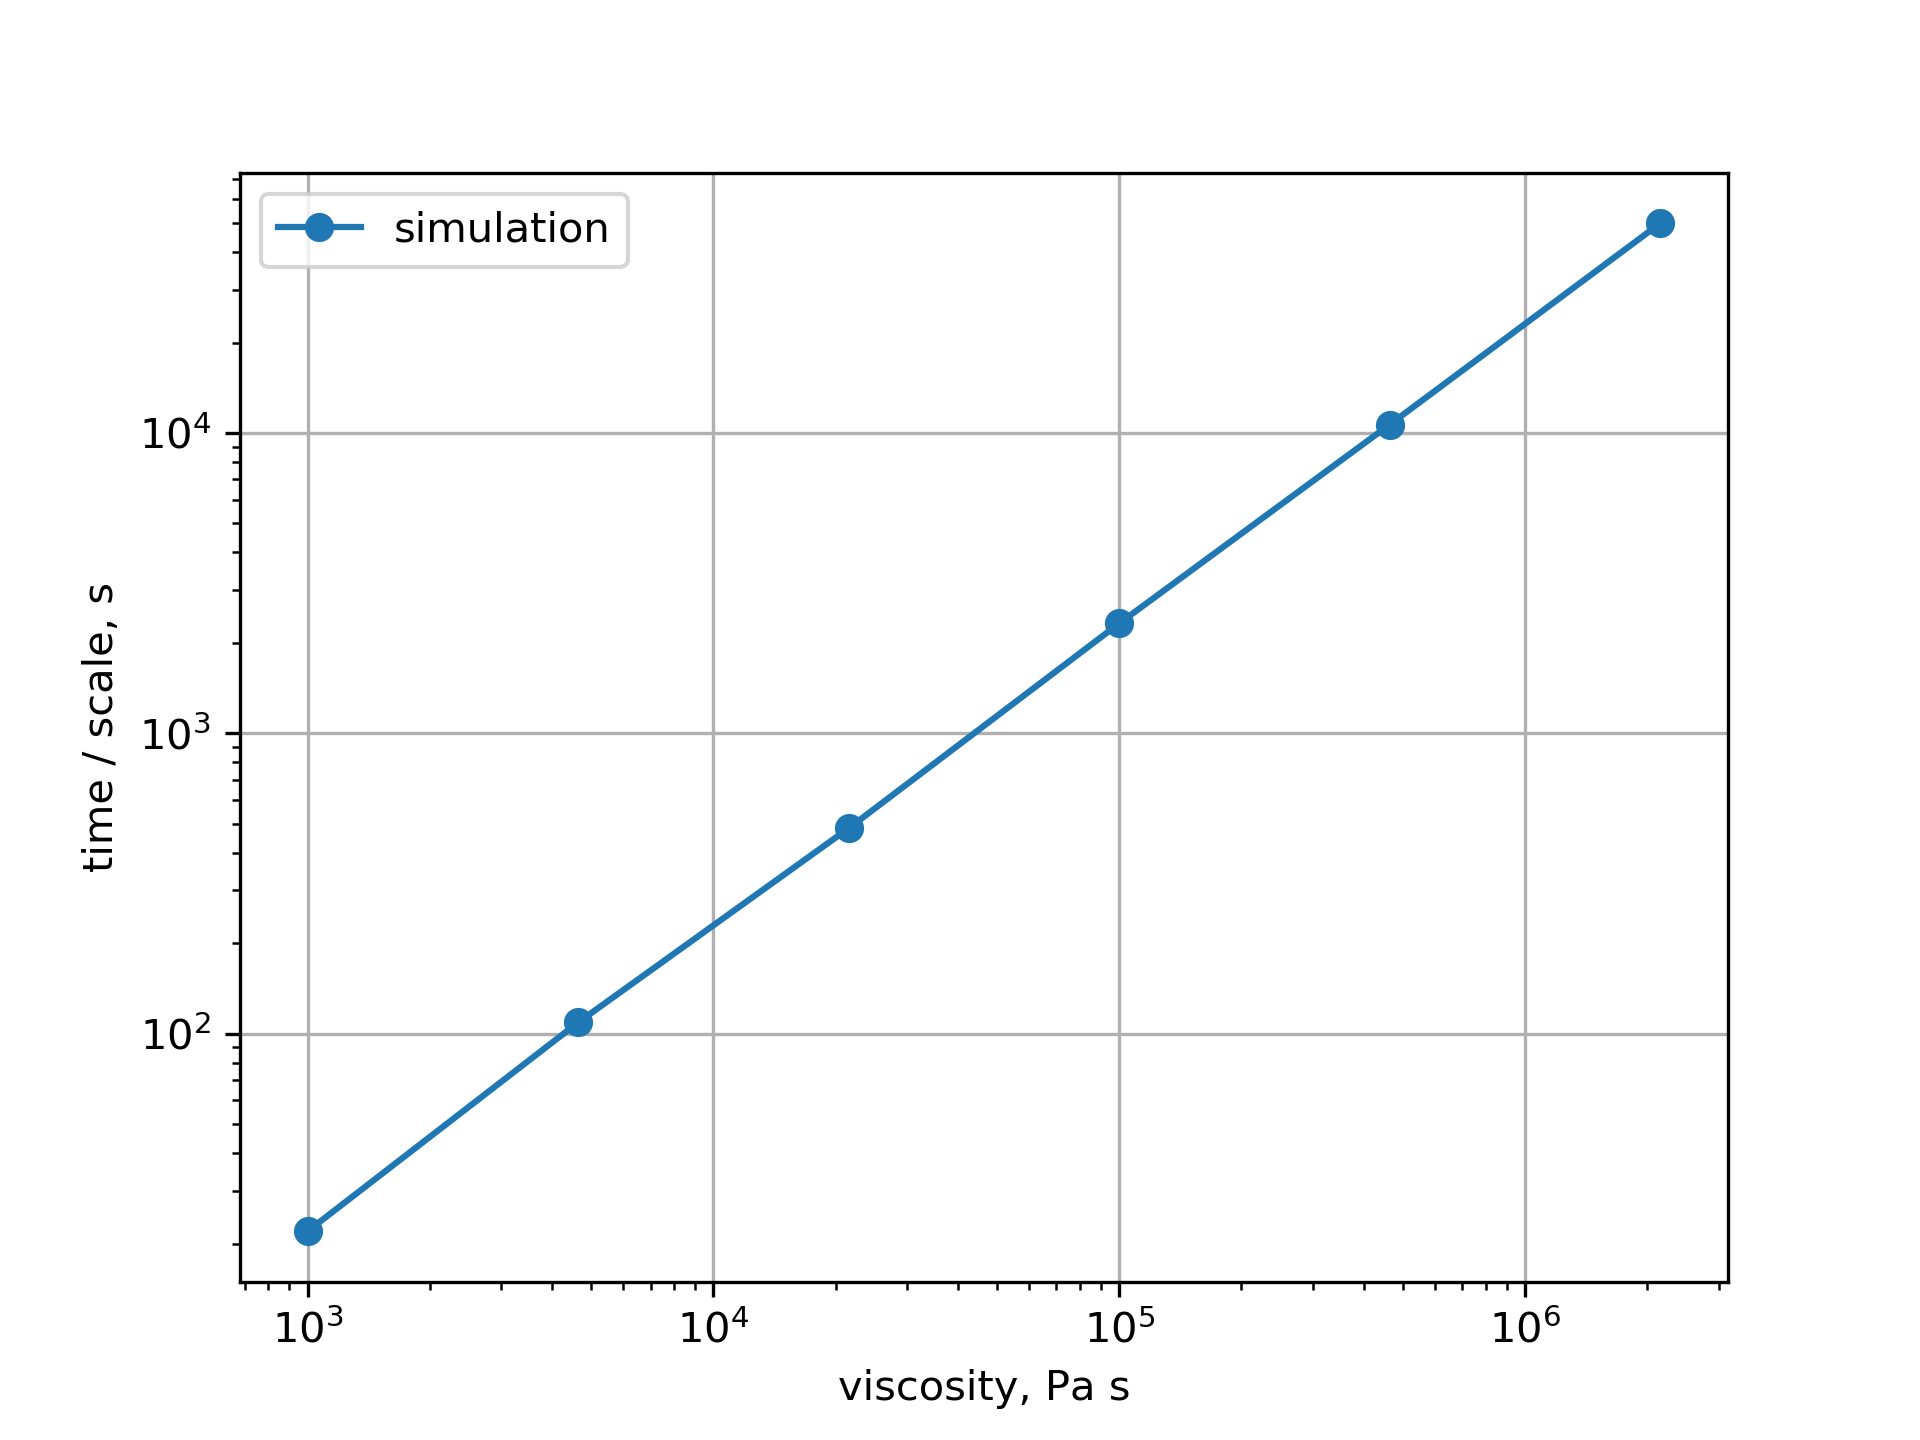
\includegraphics[width=\linewidth]{alphas} \\
	\caption{Time-\textit{scale} dependencies for different viscosity values fitted with linear function.}
	\label{fig:alphas}
\end{figure}

\begin{figure}
	\centering
	\includegraphics[width=0.6\linewidth]{С_gamma}
	\vspace{-1em}
	\caption{Linear fit of obtained $\ln(\alpha)$-$\ln(\eta)$ data.}
	\label{fig:final_fit}
\end{figure}

The determined relation between PMMA viscosity and $\alpha$ (which represents the ratio of $scale$ to $t$) enables mobility-based thermal reflow simulation by SE.
The point is that SE allows to monitor $scale$ value during the simulation, but originally $scale$ is not equal to reflow time.
The most convenient relation between $scale$ and time would be an equality ($scale \equiv t$) and it could be achieved by setting mobility equal to $\alpha$.
Indeed, if one simultaneously set
\begin{equation} \label{eq:mu_scale}
	\cases{\mu \equiv \alpha = \frac{scale}{t}, & \\
		scale = t &}
\end{equation}
the equation~\ref{eq:SE_v} doesn't change:
\begin{equation}
	\vec{\delta} = \frac{\vec{F}}{A/3} \cdot \frac{scale}{t} \cdot t \equiv \frac{\vec{F}}{A/3} \cdot scale.
\end{equation}

The equations~\ref{eq:mu_scale} is the final piece in mobility-based thermal reflow simulation of e-beam exposed PMMA.
Viscosity profile of PMMA, obtained at previous step could be easily converted into mobility profile using formula (Fig.~\ref{fig:mob_arr})
\begin{equation} \label{eq:mu_eta}
	\mu = \frac{26.142}{\eta}.
\end{equation}
Thus, one can reconstruct the surface of PMMA structure in SE, set proper mobilities of surface vertices and then run SE simulation with tracking the $scale$ factor, which will be exactly equal to reflow time.

\begin{figure}[h]
	\centering
	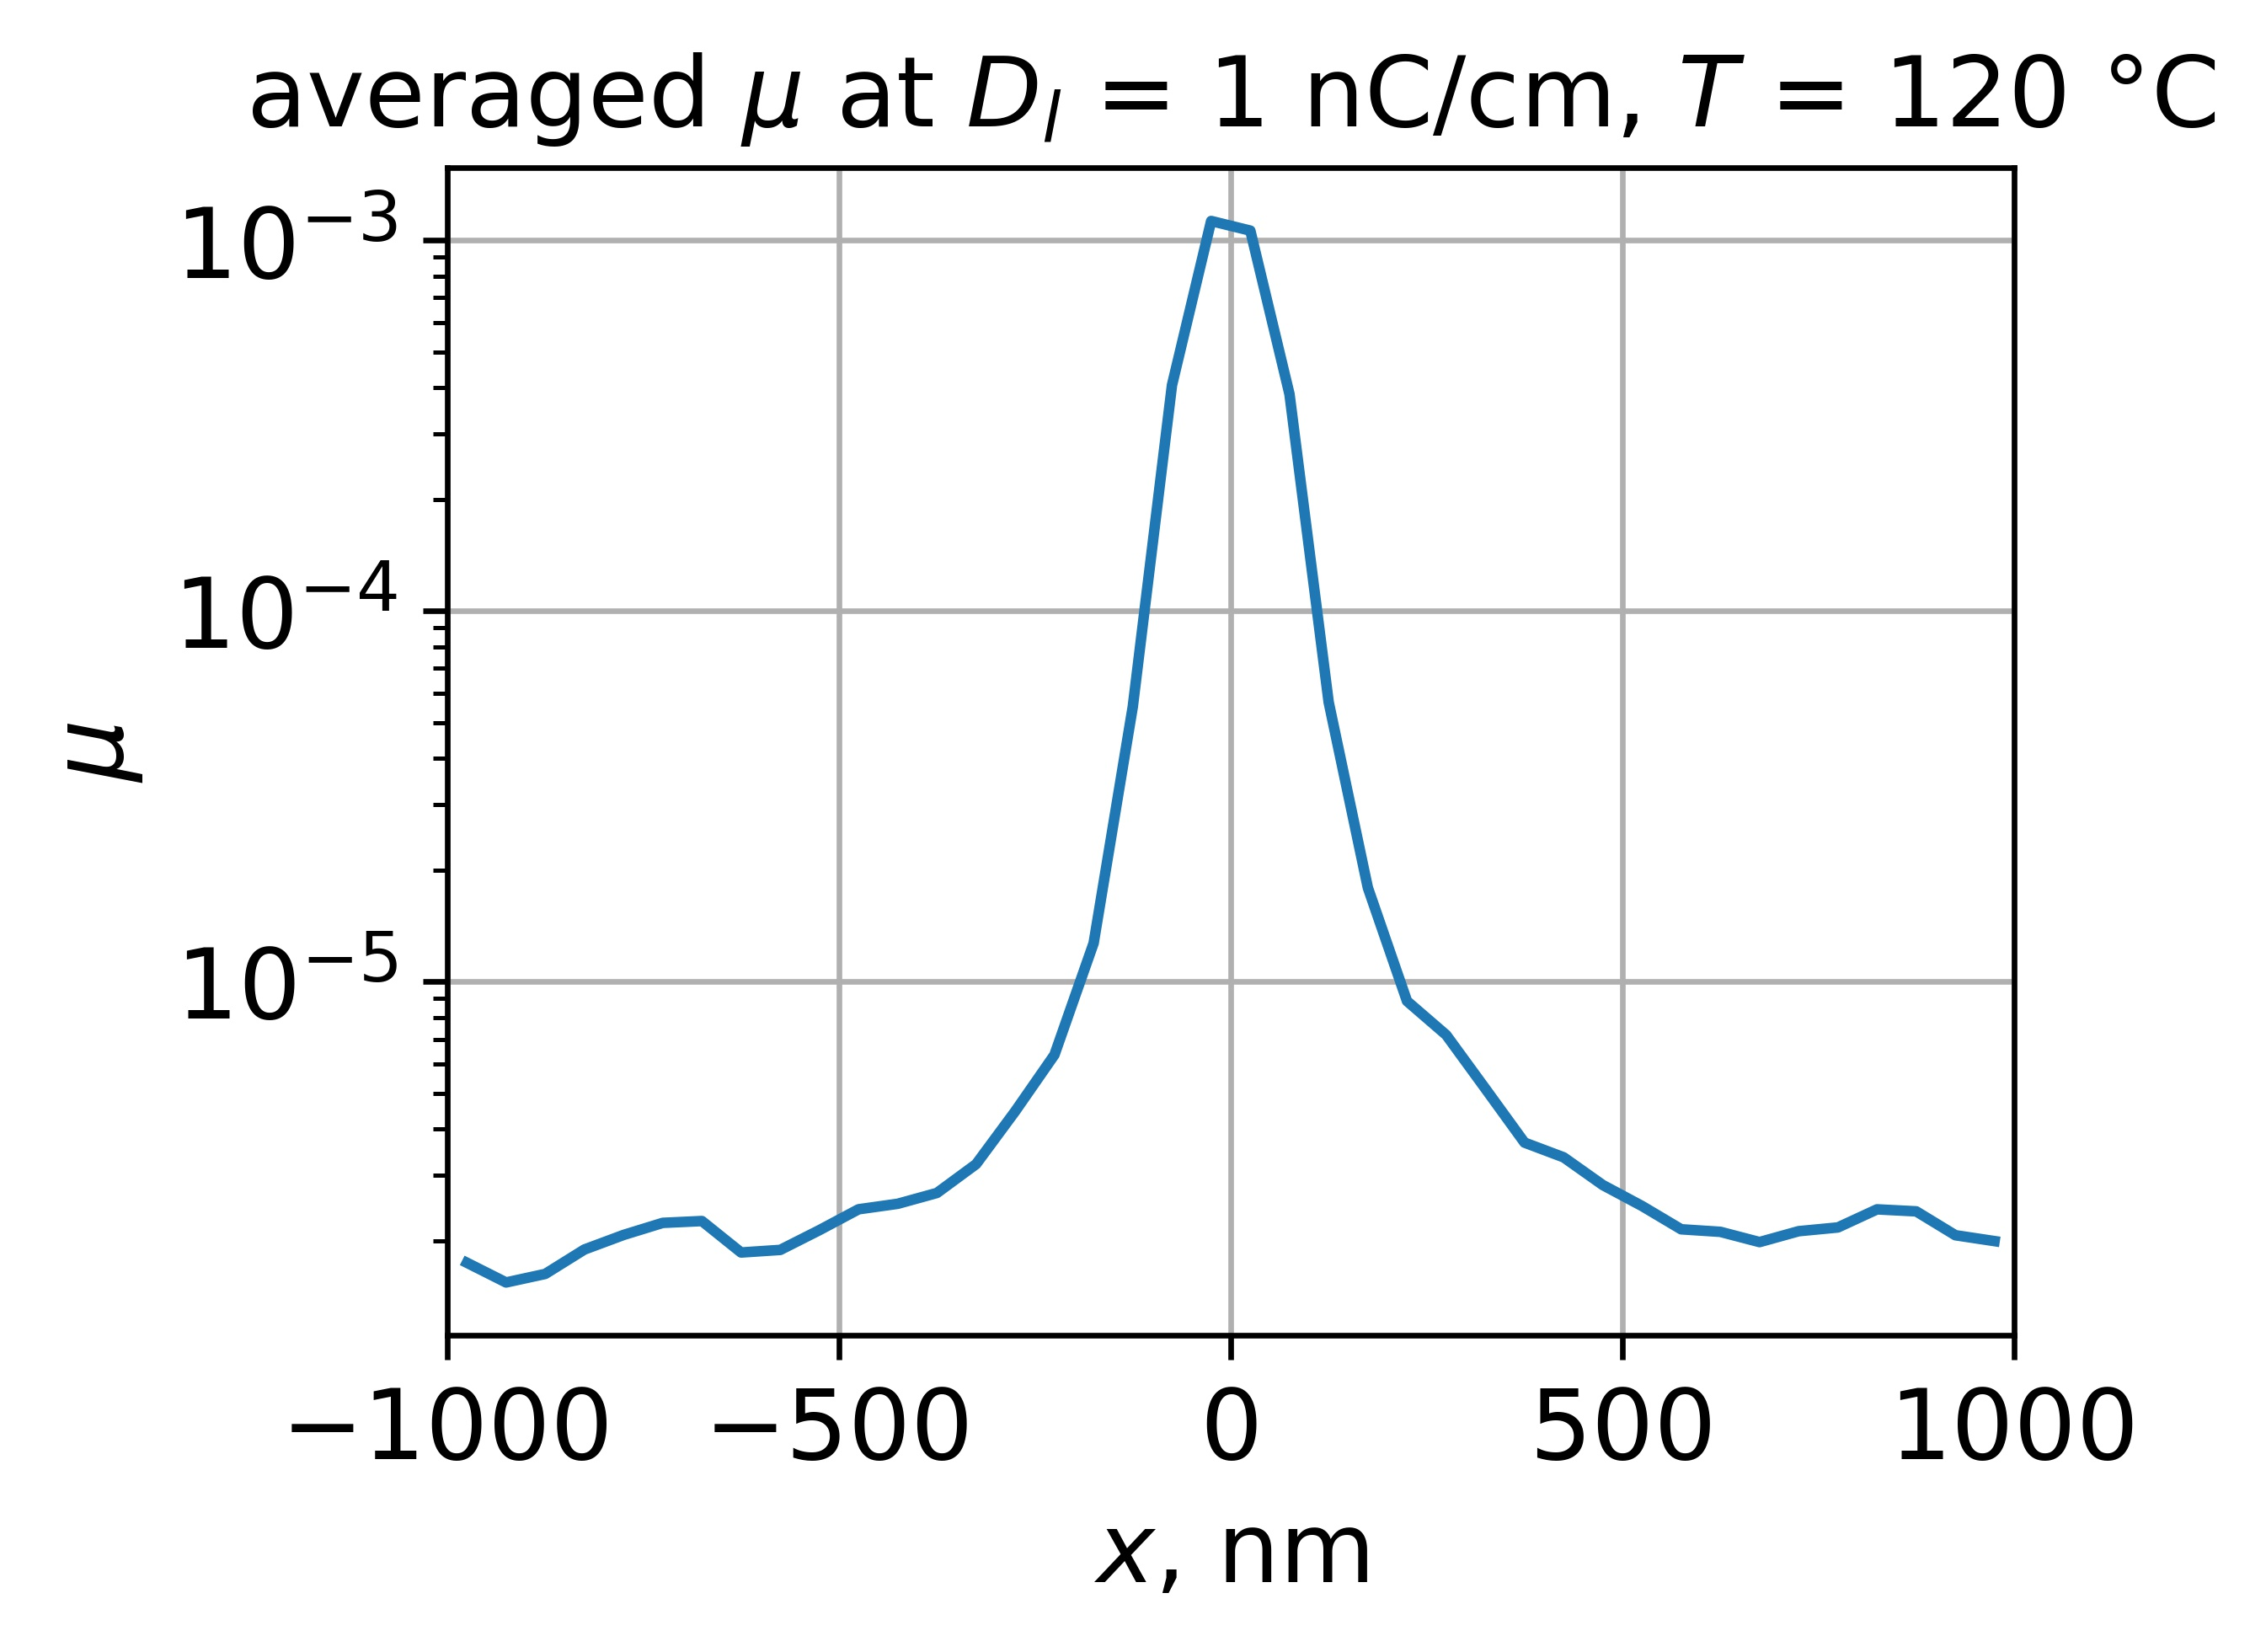
\includegraphics[width=0.6\linewidth]{mob_arr_1_nC_cm_120C_LOG}
	\vspace{-1em}
	\caption{
		Simulation of averaged (along $z$ axis) vertex mobility profile of e-beam exposed PMMA layer for 120 $^\circ$C.
		Line dose is 1 nC/cm, e-beam energy -- 20 keV, PMMA layer thickness -- 500 nm.
		Initial PMMA number average molecular weight is 271000.
	}
	\label{fig:mob_arr}
\end{figure}

\section{Discussion}

The developed method of PMMA vertex mobility determination has several remarkable features.
First, it demonstrates the agreement between reflowed profiles, simulated by analytical spectral method and ones obtained by numerical SE simulation in area normalization mode.
This emphasizes the applicability of soapfilm modeling for the simulation of polymer reflow and confirms the linear relation between $scale$ and time, proposed by Kirchner~\cite{Kirchner_SE_1}.
Moreover, the relation of inverse mobility of PMMA surface vertices and PMMA viscosity turns out to be linear too.
It is also noteworthy that developed method brings clarity into SE reflow simulation process -- in case of setting the mobilities obtained by equation~\ref{eq:mu_eta} the $scale$ factor denotes exactly the actual reflow time.

Second, this method could be applied for reflow simulation of any structure obtained in PMMA by lithographic methods.
In case profile, obtained in PMMA by grayscale e-beam lithography, simulation of PMMA main-chain scission distribution could be directly converted to PMMA viscosity profile and, finally, to PMMA vertex mobility profile.
In case of structures obtained by nanoimprint lithography the PMMA viscosity dependence on temperature and molecular weight only should be taken into account.
If sample size is much greater than structure period one can neglect the edge effects (contact angle etc.) for the reflow simulation far from sample edges.
Then structure geometry and vertex mobility distribution become the only parameters required for simulation.

Third, the described algorithm allows to expand the boundaries of thermal reflow application. At present, thermal reflow is used predominantly for profile smoothing, which not causes dramatic profile transformation~\cite{Kirchner_GL_review,Kirchner_2017}.
This results in a need for sophisticated grayscale e-beam lithography process for achievement of staircase profile close enough to required one.
The complex but predictable thermal reflow process in turn could simplify the whole fabrication method provided that greater part of profile is being formed by reflow.

\section{Conclusion} \label{conclusion}
This paper presents simulation technique for viscoelastic thermal reflow of PMMA with non-uniform viscosity profile caused by e-beam exposure with dose modulation.
Thermal reflow simulation bases on numerical search of minimal surface by finite elements method, processed by free software ``Surface Evolver'' (SE).
PMMA non-uniform viscosity profile is described by specific mobilities of PMMA surface vertices, which are embedded in surface model in SE simulation processed in area normalization mode.
PMMA surface vertex mobilities determination bases on PMMA viscosity profile which is calculated in three steps.
First, Monte-Carlo algorithm is used for the simulation e-beam induced PMMA main-chain scissions.
Then, statistical model is used to convert PMMA main-chain scission distribution to PMMA number-average molecular weight distribution.
Finally, empirical equations are used for determination of PMMA viscosity profile relying in simulated PMMA number-average molecular weight distribution
The relation between PMMA viscosity and vertex mobility of its surface was determined by simulation of rectangular grating reflow by two approaches -- analytical, based on decay simulation of profile spatial harmonics, and numerical one, processed by SE.
The obtained agreement between reflowed profiles reveal direct proportionality between SE scale factor and reflow time.
Reflow simulation in wide viscosity range resulted in turn in almost inverse proportionality between PMMA surface vertex mobility and PMMA viscosity.
Using this relation, one can calculate proper vertex mobility of PMMA structure surface vertices and process clear SE reflow simulation with scale factor denoting exactly the actual reflow time.
The developed approach could simplify complex 3D structure fabrication by deeper insight into thermal reflow processes.

\ack
The investigation was supported by the Program no. FFNN-2022-0021 of the Ministry of Science and Higher Education of Russia for Valiev Institute of Physics and Technology of RAS.


\section*{References}
\bibliography{cite_papers}

\end{document}
